\documentclass{scrartcl}
\usepackage{fontspec} %connects to native fonts
\usepackage{amsmath}
\usepackage{mathtools}
\usepackage{cleveref}
\usepackage{pgfplots}
\usepackage{graphicx}
\usepackage{wrapfig}
\usepackage{fancyref}
\usepackage{amssymb}
\usepackage{subfig}
\usepackage{float}
\usepackage[justification=RaggedRight, singlelinecheck=false, font={footnotesize}]{caption}
\usepackage[portuguese]{babel}
\usepackage[title,titletoc,toc]{appendix}


\usepackage{lipsum}
\usepackage{blindtext}
\addtokomafont{sectioning}{\rmfamily}

\begin{document}
\pagenumbering{arabic}
\bibliographystyle{plain}
\title{
	\textnormal{
	\LARGE Universidade de Lisboa - Instituto Superior Técnico\\
	\Large Licenciatura em Engenharia Informática e de Computadores\\
	\Large Análise e Síntese de Algoritmos
\\}
	\LARGE2º Projeto
	\vspace{-1ex}
	}
\author{Gonçalo Marques,
	\texttt{84719}
	\and
	Manuel Sousa,
	\texttt{84740}
}
\date{	\vspace{-1ex}
		\vspace{-4ex}
	}
\maketitle

\section*{Introdução}
Com este projeto pretendemos apresentar uma solução eficiente para o problema enunciado, explicar a sua implementação e fazer uma análise teórica e experimental da complexidade temporal e espacial do mesmo.

\section*{Descrição do problema}
O problema consiste em calcular o custo minimo de contruir um certo numero de estradas e aeroportos entre variaas cidades. As estradas sao de 2 sentidos e podem ligar pares de cidades. Cada cidade pode vir a ter um aeroporto, que pode ser utilizado como meio de transporte para outras cidades que tambem tenham aeroportos. Quer as estradas, quer os aeroportos tem um custo. Alem de calcular o custo minimo de contruir a rede de transportes que liga cidades, temos de indicar o numero de estradas e aeroportos que compooem a nossa rede mais barata, tendo sempre especial atencao, os casos em que ha varias maneiras de obter o custo minimo,ie. se varias redes com o mesmo custo (minimo) puderem ser contruidas com um numero de estradas e aeroportos diferentes, temos de preferir sempre a rede minima que controi menos aeroportos. Se nao for possivel contruir uma rede minima que inclua ligacoes a todas as cidades, entao deparamonos com uma solucao Insuficiente.

Ora este problema pode ser descrito como um problema num grafo nao dirigido, pesado, em que:
\begin{itemize}
\setlength\itemsep{-0.5ex}
\item cada cidade é um nó
\item uma estrada ou aeroporto uma aresta
\end{itemize}

Assim, o problema descrito é equivalente ao de calcular num grafo nao dirigido e pesado $G(V,E)$ (com $V = \#N$ e $E = \#A+\#S  $ , sendo $N$ o numero de cidades, $A$ o numero de cidades com aeroporto e $E$ o numero de estradas existentes entre todas as cidades), o custo total de uma arvore abrangente de menor custo.

Temos de considerar 2 situacoes. A primeira situacao consiste em ter em conta estradas e aeroportos na solucao mais ``barata''. Para representar os aeroportos no nosso grafo temos que ser ageis de forma a criar uma ligacao logica que tenha em conta as cidades com aeroportos e o custo de construir cada um deles. Por isso vamos criar um vertice adicional no nosso grafo chamado "Cidade Aerea", onde todas as cidades que possam ter um aeroporto se ligam. Como todas as cidades com aeroportos se ligam ao mesmo vertice ficam ligadas entre si, sendo o custo de um aeroporto registado em cada uma das arestas, nao ha trabalho adicional no calculo do custo da miniminm spaning tree. A segunda situacao consiste em calcular o custo minimo apenas numa solucao com estradas. Neste caso ignoramos por completo os aeroportos (retirando-os do grafo), e calculamos o custo minimo de constuir uma rede. Por fim, a solucao final sera o menor custo de ambas as situacoes.

Antes de ter em conta cada umas das 2 situacoes temos de nos preocupar com a connectividade do grafo, pois se o grafo nao for ligado entao nunca vamos conseguir calcular uma rede que engloba todas as cidades, visto que ha pelo menos um conjunto de cidades que nao tera ligacoes para as restantes.

\section*{Algoritmo utilizado}
Tendo a solução do problema sido estudada nas aulas, foi utilizado o algoritmo estudado - o algoritmo de calculo da minimum spanning tree, Prim. Para contruir uma solucao bastante eficiente, contruimos uma Fibonacci Heap para reduzir os temos de acesso na fila de prioridades utilizada pelo algoritmo de Prim.

\section*{Estruturas utilizadas:}
\begin{itemize}
\setlength\itemsep{-0.5ex}
\item \textbf{G[$u$][i]} - O grafo $G$ foi representado como uma lista de adjacências (foi utilizado um std::vector (array dinâmica) em vez de std::list (lista duplamente ligada), pelo facto de a implementação do std::vector ser bastante mais eficiente que a de std::list \cite{ISOC++:2003}).
\item \textbf{visited[$u$]} - O nó $u$ foi visitado?
\item \textbf{taken[$u$]} - O nó $u$ foi ligado na minimum spanning tree?
\item \textbf{heap} - Fibonnacci Heap utilizada pelo Prim
\end{itemize}
Todas estas estruturas (com excecao da Fibonnacci heap) foram implementadas com o std::vector de C++ que tem tempo de inserção no fim $O(1+)$ e de acesso $O(1)$. Com tempo de inserção $O(1+)$ (constante amortizado), queremos dizer que para inserir $N$ elementos a complexidade de pior caso é $O(N)$, apesar da complexidade de pior caso de inserção de 1 elemento não ser $O(1)$ (de facto é também $O(N)$). \cite{ISOC++:2003}

\section*{Explicação do algoritmo}
 Para o caso de um grafo dirigido com pelo menos 2 nós, é executada uma pesquisa em profundidade ao longo dos nós, a partir do nó 1. Para cada nó visitado na DFS é guardada informação relativa ao seu estado de visita (vetor visited). Depois para cada nó, chama o ciclo DFS a todos os nós adjacentes não visitados. Quando a pesquisa em profundidade terminar, correremos de forma linear o nosso vetor visited por forma a encontrar um vertice que nao tinha sido visitado durante a pesquisa. Se isso acontecer


Primeiro construimos o grafo que contem as estradas a ligar cidades e os aeroportos que estao a ligar a "cidade Aerea", e verificamos a sua connectividade. Se o grafo nao for conexo entao estamos perante uma solucao "Insuficiente" isto porque se o grafo nao for conexo com as ligacoes das estradas e dos aeroportos, entao tambem nao sera conexo se so composta com estradas. Se o grafo for conexo, entao reunimos as condicoes para calcular o custo total da arvore abrangente de menor custo. , aplicamos o algoritmo de Prim  para calcular o custo minimo da nossa rede, assim como o numero de aeroportos e estradas que compoem essa mesma rede.

EXPLICAR PRIM


Por fim contruimos o grafo que compoe apenas as ligacoes das estradas entre cidades



 \cite{dfs:CLRS}


\section*{Análise assintótica temporal teórica do algoritmo}

Para verificarmos a connectividade de um grafo, chamamos a funcao de DFS apenas 1 vez com inicio num no arbitrario (ao contrario de uma pesquisa em profundidade normal que chama a funcao DFS em todos os nos do grafo). O objetivo disto e visitar todos os vertices de um grafo com inicio num no arbritrario. Se o grafo nao for todo visitado, entao o grafo e desconexo. Como percorremos todos os nós adjacentes a um certo nó, dentro de uma chamada DFS, podemos concluir que a complexidade de todas as chamadas pode ser descrita como $\ \sum_{i=1}^{N} \#G[i] = L$. Assim, a complexidade desta verificacao neste caso é no pior caso $O(max(N,L))$ = $O(N+L)$ que equivale a percorrer o grafo todo. Visto isto, se tivermos um grafo muito denso ou seja com $L \gg N$, a DFS correra em $O(L)$ e $O(N)$ se muito esparco, isto e se $N \gg L$.

Para calcular o custo total da arvore abrangente de menor custo, teremos de correr o algoritmo de Prim. Dado que com Fibonacci Heap como fila de prioridades conseguimos tempos de insercao e de Decrease-Key de $O(1+)$ (constante amortizado). Para escolher a aresta com o peso mais baixo teremos $O(log(E)) = O(log(V))$ (amortizado) visto que se $E = V^2$ temos $log(E) = log(V^2) \equiv 2Log(V) = O(log(V))$.Concluimos entao que a complexidade total do algoritmo de Prim com Fibonacci Heap como fila de prioridades sera de $O(E + V log V)$.

Concluímos então que teremos sempre complexidade de melhor e pior caso $O(E + V log V)$ se um dos grafo contruido numa das 2 situacoes (descritas na discricao do problema) for conexo. Se nenhum dos grafos for conexo, entao a complexidade do algoritmo fica limitada a complexidade de verficicacao de connectividade, ou seja $O(max(N,L))$ = $O(N+L)$ (caso geral).

\section*{Binary Heap V.s Fibonacci Heap}

O uso de Fibonacci Heap como fila de prioridades tras claras vantagens de eficiencia na resolucao deste problema em comparacao por exemplo com uma Binary Heap que tem tempo de insercao de $O(log(E)) = O(log(V))$, contra $O(1+)$ (constante amortizada) da Fibonacci Heap. Com uma Binary Heap, escolher a aresta com o custo mais baixo custa $O(log(E)) = O(log(V))$. Portanto a compolexidade final de Binary Heap seria $O(Vlog(V) + Elog(V)) =  O(Elog(V)$, que e bastante pior (para grafos muito densos) em comparacao com a complexidade de $O(E + V log V)$ ($O(E)$ para grafos muito densos) da Fibonacci Heap.

Provavmos assim que a utilizacao de Fibonacci Heap como fila de prioridades, torna a solucao significativamente mais rapida em termos de eficiencia.


\section*{Análise assintótica espacial}
Como se verifica pelas estruturas utilizadas, o algoritmo utiliza 2 estruturas com $N$ booleanos (visited e taken), e uma estrutura com $N$ vetores, mas com o total de $L$ arestas (representadas com std::pair, sendo o pair <custo,vertice de ligacao>) no seu interior. Como e tudo guardado sobre variaveis locais podemos conluir que a memória de stack tem complexidade de pior caso $O(N+L)$, que e o custo de representar o grafo. Dado que a Fibonaccy Heap nao guarda mais que $O(N+L)$ elementos, nao influencia o pior caso da complexidade espacial.


\section*{Análise assintótica temporal experimental do algoritmo}
\begin{wrapfigure}{r}{0.5\textwidth} %this figure will be at the right
	\centering
	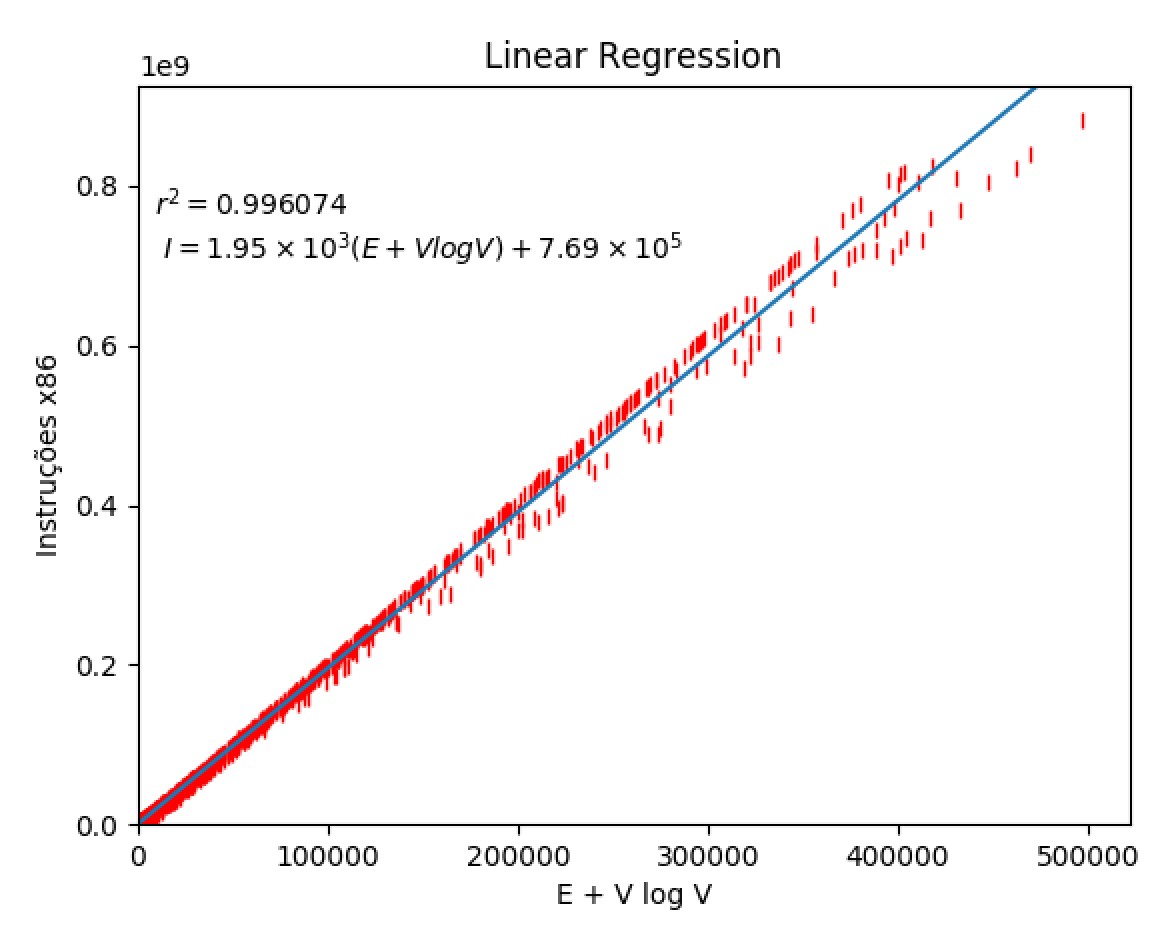
\includegraphics[width=0.4\textwidth]{images/analise.png}
	\caption{Análise experimental com parâmetros $2 \le N \le 10000 $ (1000 riscos)}
	\label{fig:analexp}
\end{wrapfigure}
Para se realizar a análise experimental temporal do algoritmo, foi utilizada a aproximação que cada instrução de C corresponde em média a um número fixo de instruções de CPU. Assim, em primeiro lugar procedeu-se à geração de $K$ diferentes casos de teste aleatórios para uma das soluções possíveis, também escolhidas aleatoriamente (para cada caso foi escolhido aleatoriamente um $N$ e um $L\ge N-1$). De seguida, para cada caso de teste foi utilizada a ferramenta perf para contar o número de instruções de CPU utilizadas em modo utilizador durante a execução do programa - $I$. Por fim, fez-se o plot do gráfico de $I$ em função de $N+L$. Obteve-se assim os resultados da Figura \ref{fig:analexp}.\par
Sendo o coeficiente de correlação linear muito próximo de 1, a análise experimental comprova o resultado teórico esperado.

\bibliography{ref}

\end{document}
